
\documentclass[11pt]{article}
\usepackage[lmargin=0.5in, rmargin=0.5in,tmargin=1.0in,bmargin=1.0in]{geometry}
\usepackage{graphicx}
\usepackage{times}
\title{Physics Behind the Simulation: A CS296 Report by Group 31}
\author{Sai Charan\\
  120050060\\
  \texttt{saicharan@iitb.ac.in}\and
  Vinay Chandra\\
  120050063\\
  \texttt{vinaychandra@iitb.ac.in}\and
  Nikhil Sri Ram\\
  120050070\\
  \texttt{nikhil007@iitb.ac.in}\\
}
\date{\today}

\begin{document}

\maketitle
\section{Introduction}
Box2D [4] is a 2D rigid body simulation library for games.It is a physics engine written in C++ for animation.\\
It is using this library we tried to portray the mechanism involved in working of a had gun as our course project.In this report we explain the working and physics involved in the project with a insight on timing and performance of the code.
\section{Our initial design prototype}
\begin{center}
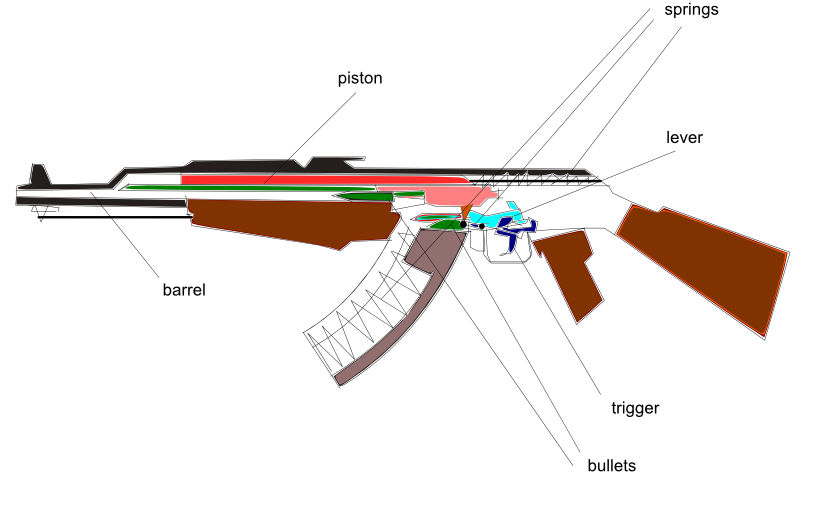
\includegraphics[scale=0.7]{../details/images/2.png}
\end{center}
\section{Final Simulation}
\begin{center}
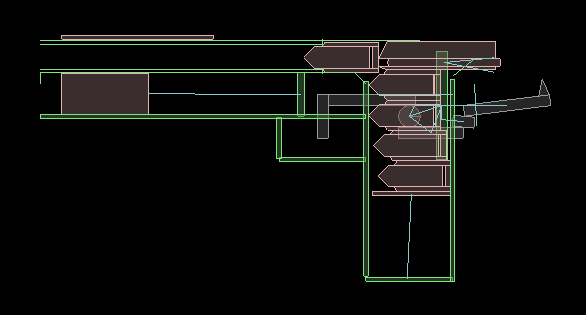
\includegraphics[scale=0.7]{../details/images/gun.png}
\end{center}
\section{Objects in simulation}
The whole simulation can be broken down to four parts:-
\begin{enumerate}
\item Static skeleton of gun
\item The dynamic encasing around the skeleton
\item Bullets and the catridge system
\item Trigger part
\end{enumerate}
\subsection{Static skeleton of gun}
Built using the static bodies \cite{box2d}
this part forms the rigid skeleton part of the gun.The part includes tunnel for the bullet and space for the hammer part.It also includes the enclosing for the catridge area. In a nut shell it is skeleton but itself is immovable, Refer to figure 1 below.
\begin{figure}[here]
\begin{center}
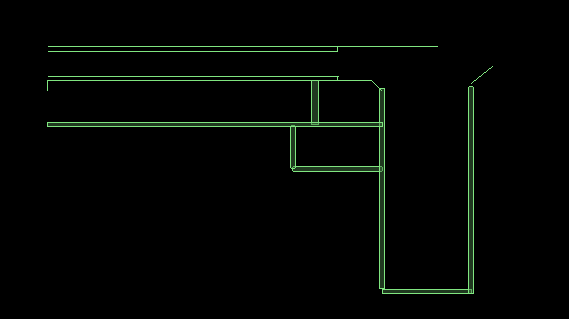
\includegraphics[scale=0.3]{../details/images/static.png}
\caption{skeleton}
\end{center}
\end{figure}
\subsection{The dynamic encasing around the skeleton}
\begin{figure}[here]
\begin{center}
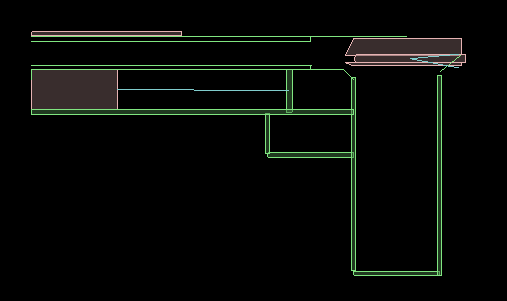
\includegraphics[scale=0.3]{../details/images/stick.png}
\caption{encasing}
\end{center}
\end{figure}
This part of the gun mainly consists of two fixtures \cite{box2d}
embedded on a dynamic body  \cite{box2d}
\begin{enumerate}
\item A : \\
It is the part below the bullet tunnel and is responsible for the reloading simulation of the gun.The reloading part is carried out by the spring (implemented by the distance joint \cite{box2d}
) whose one end is connected to this part and the other to the static part of the gun.
\item B: \\
This part is the part that pushes the bullet to the point where they are triggered .It also contains the firing pin responsible for the explosion which is held in its place with the help of two springs between the pin and the outer casing.
\end{enumerate}
\subsection{Bullet and the catridge system}
\begin{figure}[here]
\begin{center}
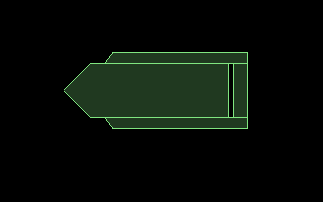
\includegraphics[scale=0.3]{../details/images/bullet.png}
\caption{bullet}
\end{center}
\end{figure}
The bullet itself consists of two fixtures \cite{box2d}
one the bullet itself and second is the encasing around the bullet which is shelled out during reloading.Both the parts hold on two each other due to the enormous friction between likewise in the reality.\\
\begin{figure}[here]
\begin{center}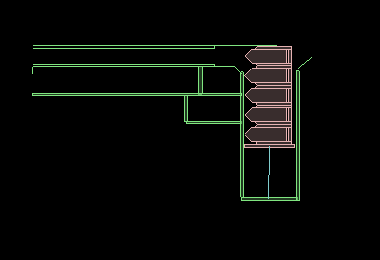
\includegraphics[scale=0.3]{../details/images/bullets.png}
\caption{skeleton with catridge}
\end{center}
\end{figure}\\
The catridge system consists of a base over which the bullets are stacked one upon other.Also note that there is a spring joining the base to the skeleton which is responsible for pushing the bullets up once the bullet above is used up.
\subsection{The trigger part}
\begin{figure}[here]
\begin{center}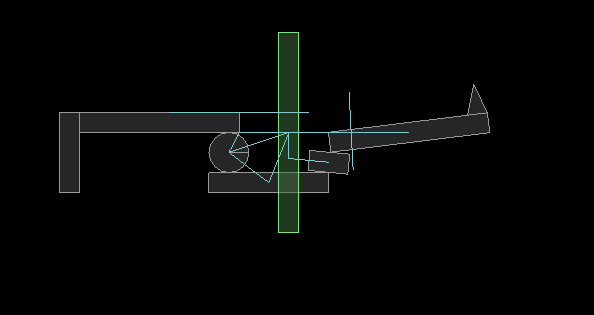
\includegraphics[scale=0.3]{../details/images/trigger.png}
\caption{the trigger part (seperated)}
\end{center}
\end{figure}


The above figure depicts the mechanism involved in the trigger part of the gun.This part is grouped \cite{box2d}
such that it does not interfere with the rest of the body. This can be thought of as the two parts are in space with same 2d coordinates but one behind the other.\\
   Coming the parts of the system, it consists of a static body (say S) to which all the references are taken and springs are attached. There are two rods (\bf R1 \rm and \bf R2 \rm ) sliding over the surface of the circle which acts as a gear. Of these two rods one rod is directly connected to the trigger (\bf R1\rm). Notice the spring between \bf R1 \rm and \bf S \rm  which brings back \bf R1\rm to its position once the trigger is pulled. Next there is flap (\bf F\rm) tied to \bf S \rm with the help of a revolute joint\cite{box2d}
The body that rests over the \bf F \rm is the hammer part, \bf H \rm, that actually hits the firing pin in the process. The flap can be thought of as a lock preventing \bf H \rm from hitting pin. There is a spring attached to \bf H \rm which provides it momentum enough to hit.
\section{Explanation to the physics of simulation}
The Explanation to the whole simulation can be summarised as follows:-\\
    Once the trigger (R1) is pushed , R2 moves back because of the presence of a gear which release flap. Releasing the flap inturn releases the hammer (\bf H \rm) which moves around the revolute joint and hits the firing pin. When the collision between the firing pin and hammer is recorded, the explosion event is invoked. This explosion event imparts momentum to the bullet in the forward direction and while a backward momentum to the B and casing simulataneously which pushes B and casing backward. \\ Meanwhile, the flap is brought into its position because of the spring present between \bf R1 \rm and \bf S. \rm As B moves backward, it pushes H to its initial position and H gets locked up above the flap. In the due course, next bullet gets pushed up filling up the empty space above it.
\section{Observations}
\subsection{Average step time, Average loop time vs Iteration no.}
The average step time decreases with the number of iterations, whereas the average loop time increases in a non-linear way.
\begin{center}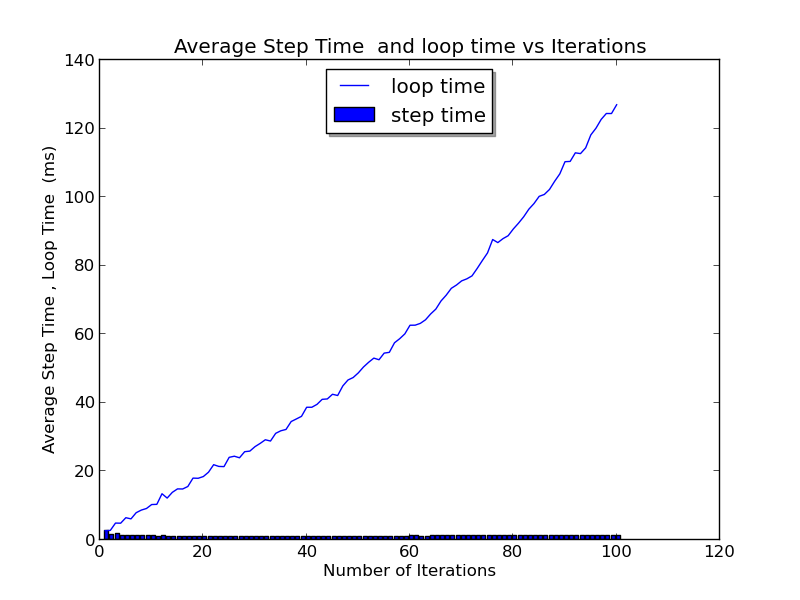
\includegraphics[scale=0.7]{../details/images/g31_plot01.png}
\end{center}
The average step time decreases with the number of iterations as opposed to the intuition where we assumed that it should stay constant with the iter no.This can be seen as the time taken for the execution step time can be divided to time taken for calling the function which includes time for locating the function in the code etc.,(say t1) and the actual time for the execution of step time(say t2).t2 is linearly proprtional to number of iterations while t1 is remains almost constant for any number of iterations.therfore the value of t1 average for iterations decreases and therefore the steptime on an whole decreases. whereas the average loop time increases in a non-linear way.\newline
whereas the loop time increases with the iteration value which is fairly clear as iternumber increases number of times code goes into the loop increases and therefore the time (looptime) increases.However the graph does not follow a regular linear trend which can be attributed to time for access (as t2 in the above case) and also for the nonlinearity in the system itself.


\subsection{Collision, position and velocity updates vs Iteration no.}
1. From the plot, it is clear that both position updates and collision time follow almost similar graph.\newline
2. velocity updates take more time than position updates.\newline
3. $steptime$ is higher than update sum throughout the graph
\begin{center}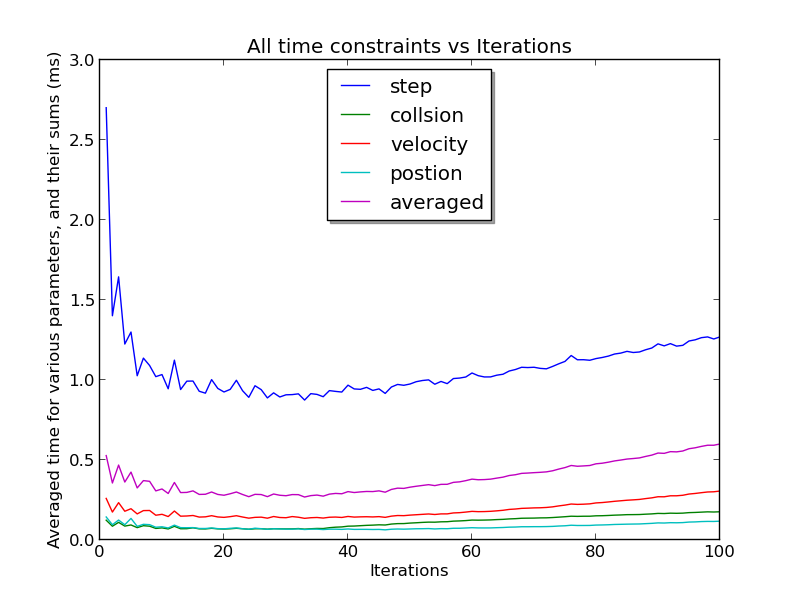
\includegraphics[scale=0.6]{../details/images/g31_plot02.png}
\end{center}

The plot for position updates and collision time being similar across all iter numbers gives us a hint that job done by both these functions is somehow similar which is infact in true in a sense.collision time refers to what are the collisions occuring and between what objects which in a way is infact dependent on the positions of the objects.\newline
Secondly, velocity updates is always higher than the graph for collision and position update time.This is because the number of equations involved in calculating velocities of individual objects involve more equations than for positions and therefore require more time.\newline
Third,the step time is higher than update sum.This is because step time covers all the updates plus some extra processes other than the updates and therefore always remains higher.

\subsection{Step time vs Iteration no.}
Errors in step time decreases with iteration no.
\begin{center}
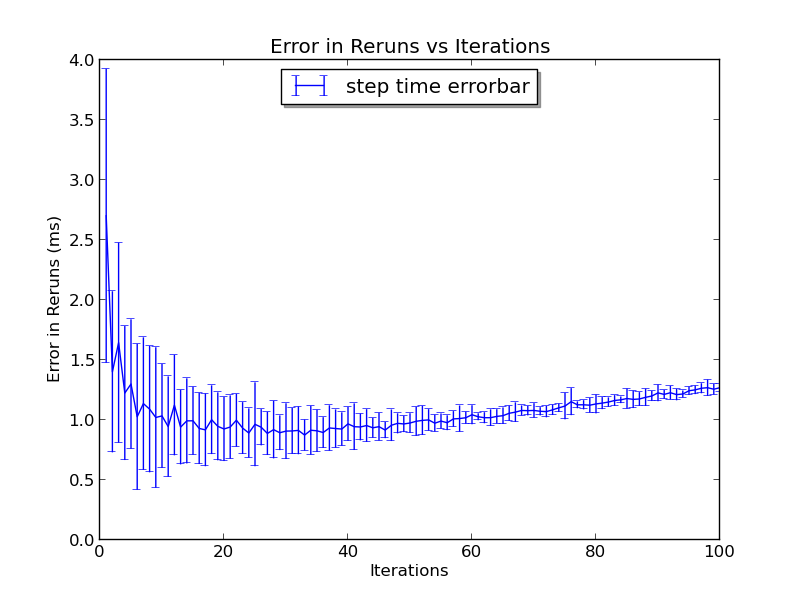
\includegraphics[scale=0.6]{../details/images/g31_plot03.png}
\end{center}

Errors in step time decreases with iteration no.This is on par with our intution that the devation in any random outcome (like the noise) decreases with the number of times the experiment is performed and therefore the trend.\newline


\subsection{Frequency of step time variation}
The graph appears to be a Heavy-tailed Gaussian distribution.
\begin{center}
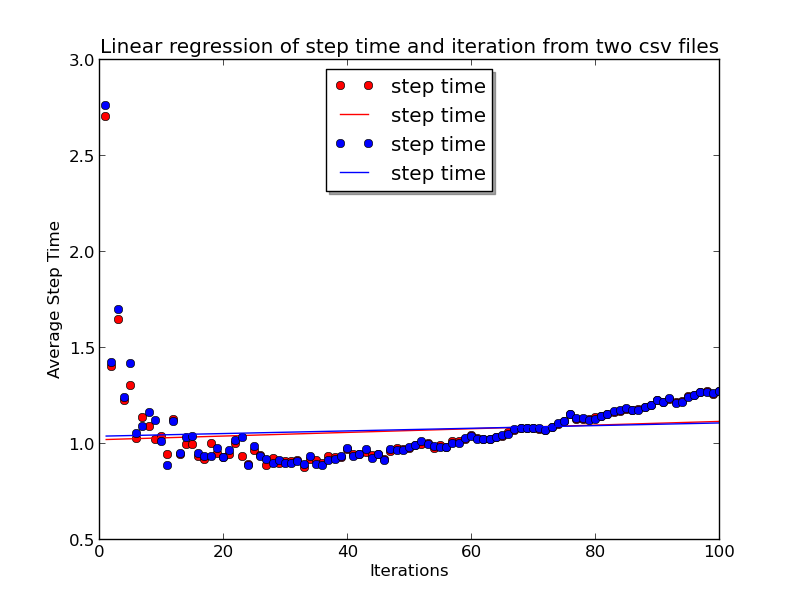
\includegraphics[scale=0.6]{../details/images/g31_plot04.png}
\end{center}

\section{Profiling}
We first ran the executable first with the compiled version of box2D using release (say case 1) and later with debug (say case 2).While doing so for release we included -On flag and for the other we omitted the flag.Inorder to observe the profile we chose the value ITER as 100000.
\subsection{Obsevation}
By looking the data,we notice that the number of functions called for in case 1 is lower than the number of functions called for in the case 2.The prime difference is that we included -O3 in tcase 1 and in case we did not.-O3 (any -On), is the flag for the optimization.\newline
Which implies our base Box2d code is not optimized in the case 2 as it is in case 1.Therefore the execution in case 2 takes more time resulting a lot of calls to the functions of which many of them turns to be useless.For instance with the iter value = ITER , the number of functions called in the case 1 is 193 compared to 157 in case 2.\newline
Inorder to see which of these functions are redundant or which of them can be optimised we look into the corresponding .dat files\newline
we observe that the function \it b2Vec2::b2Vec2(float, float) \rm which is appearing most number of times in the case 2 is absent in case 1 and therefore is redundant and conclusion can be that the equivalent process can be carried out without putting any extra call to the function as done in the case 1.\newline
Also, functions like b2Mul,b2Dot etc., follow the same trend.
for more on profiling \cite{gprof}

\section{Call Graph}
The call graph included is for exectuable with Iter value = 100000 compiled with Debug implementaion (without -O3 flag) of 
\begin{center}
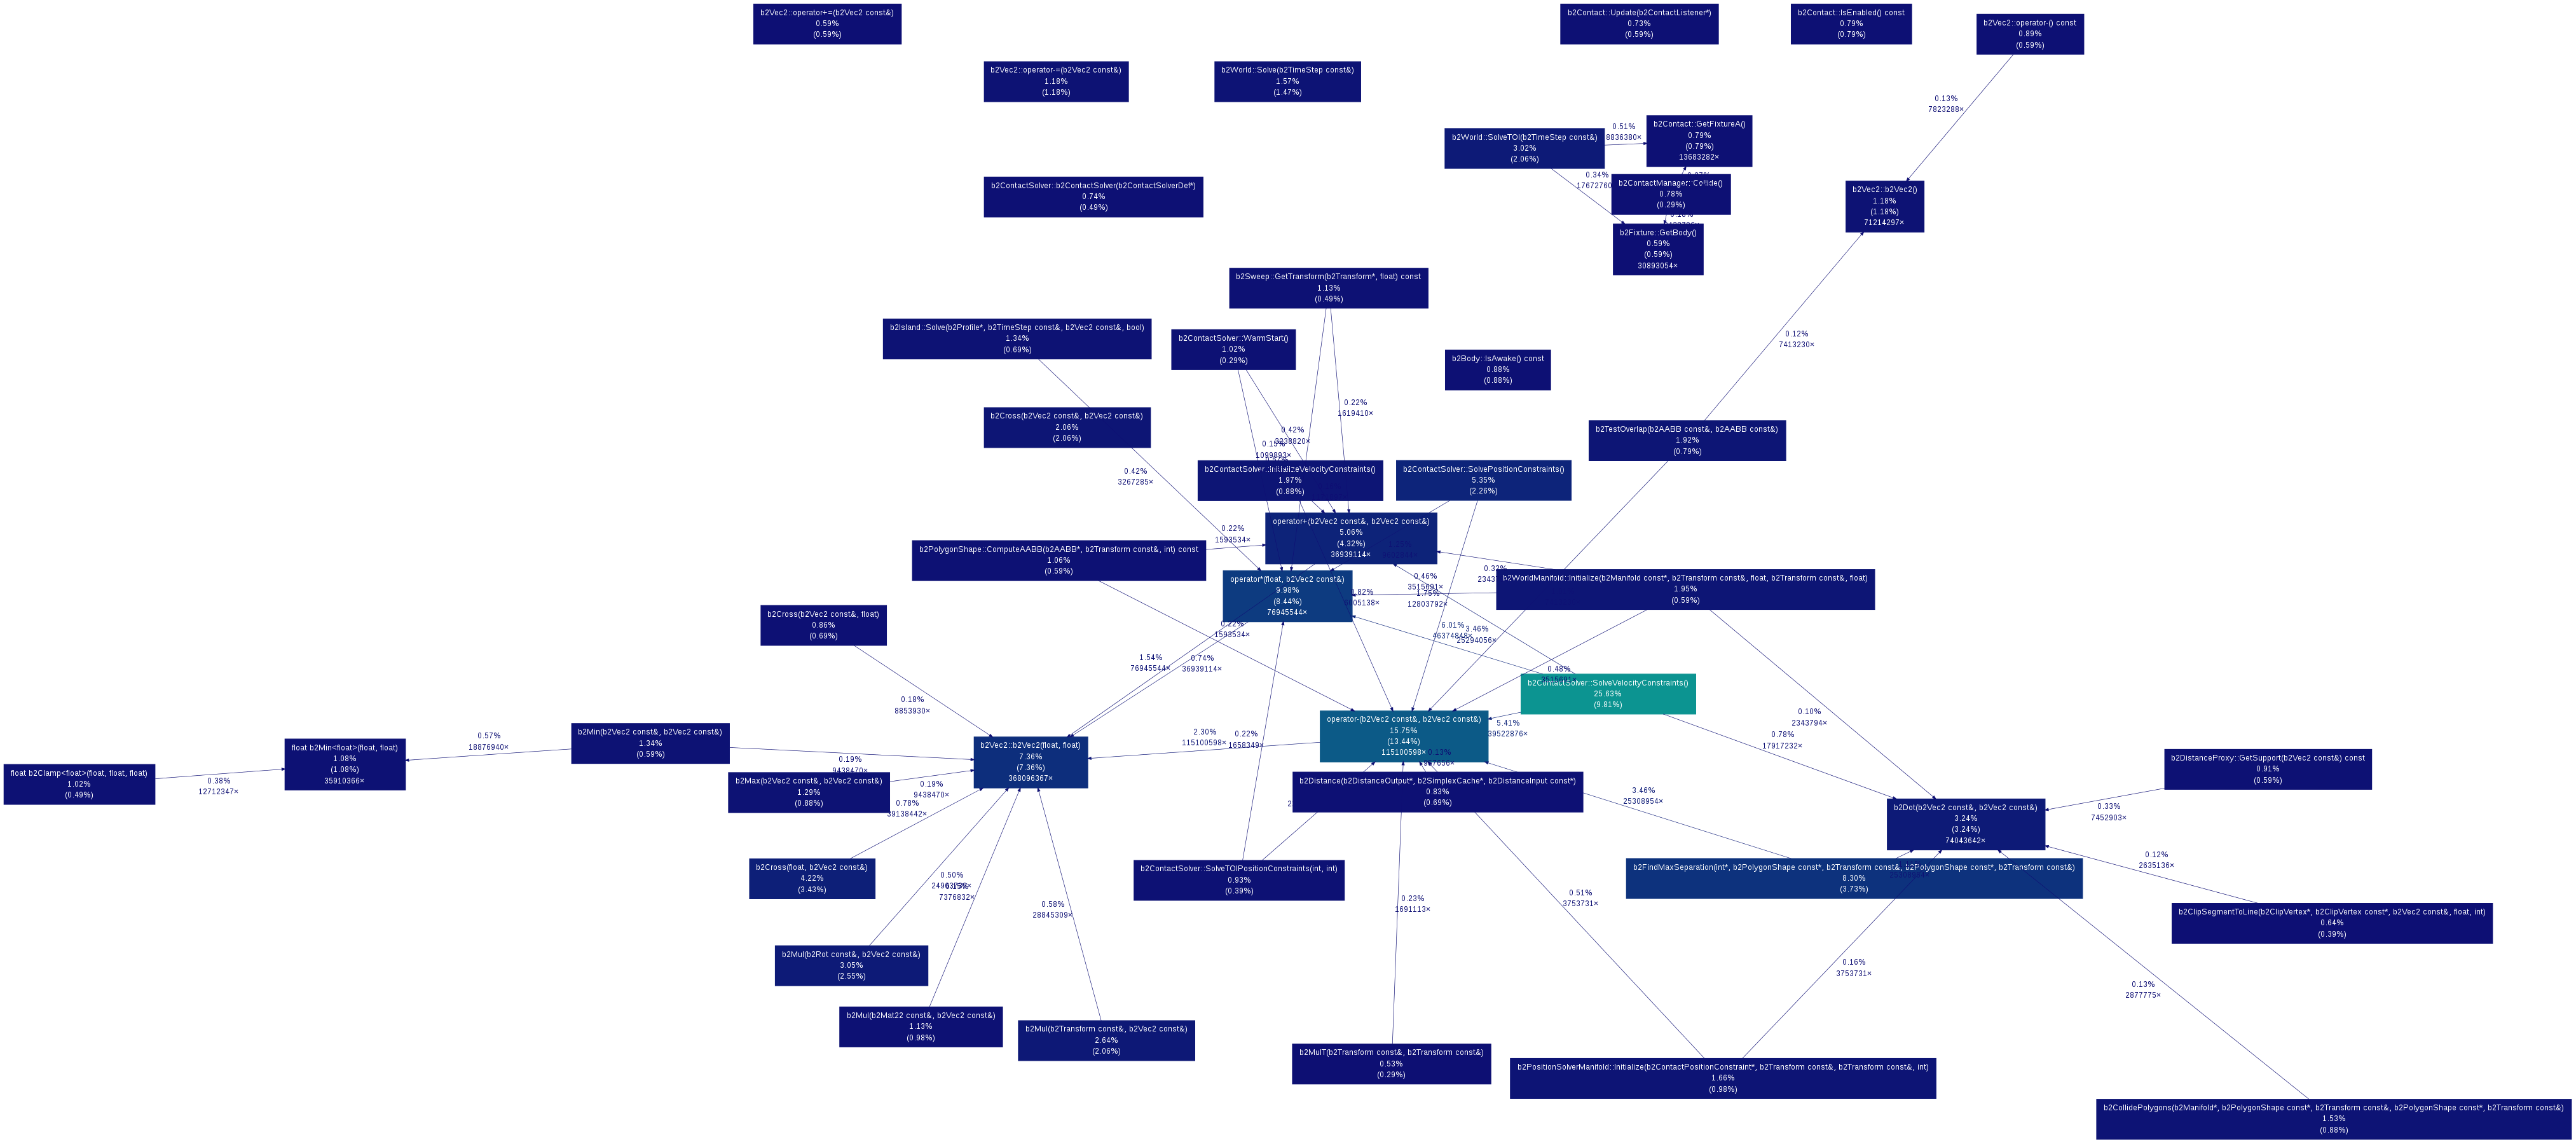
\includegraphics[scale=0.1]{../details/images/debug.png}
\end{center}
for release implementation\\
\begin{center}
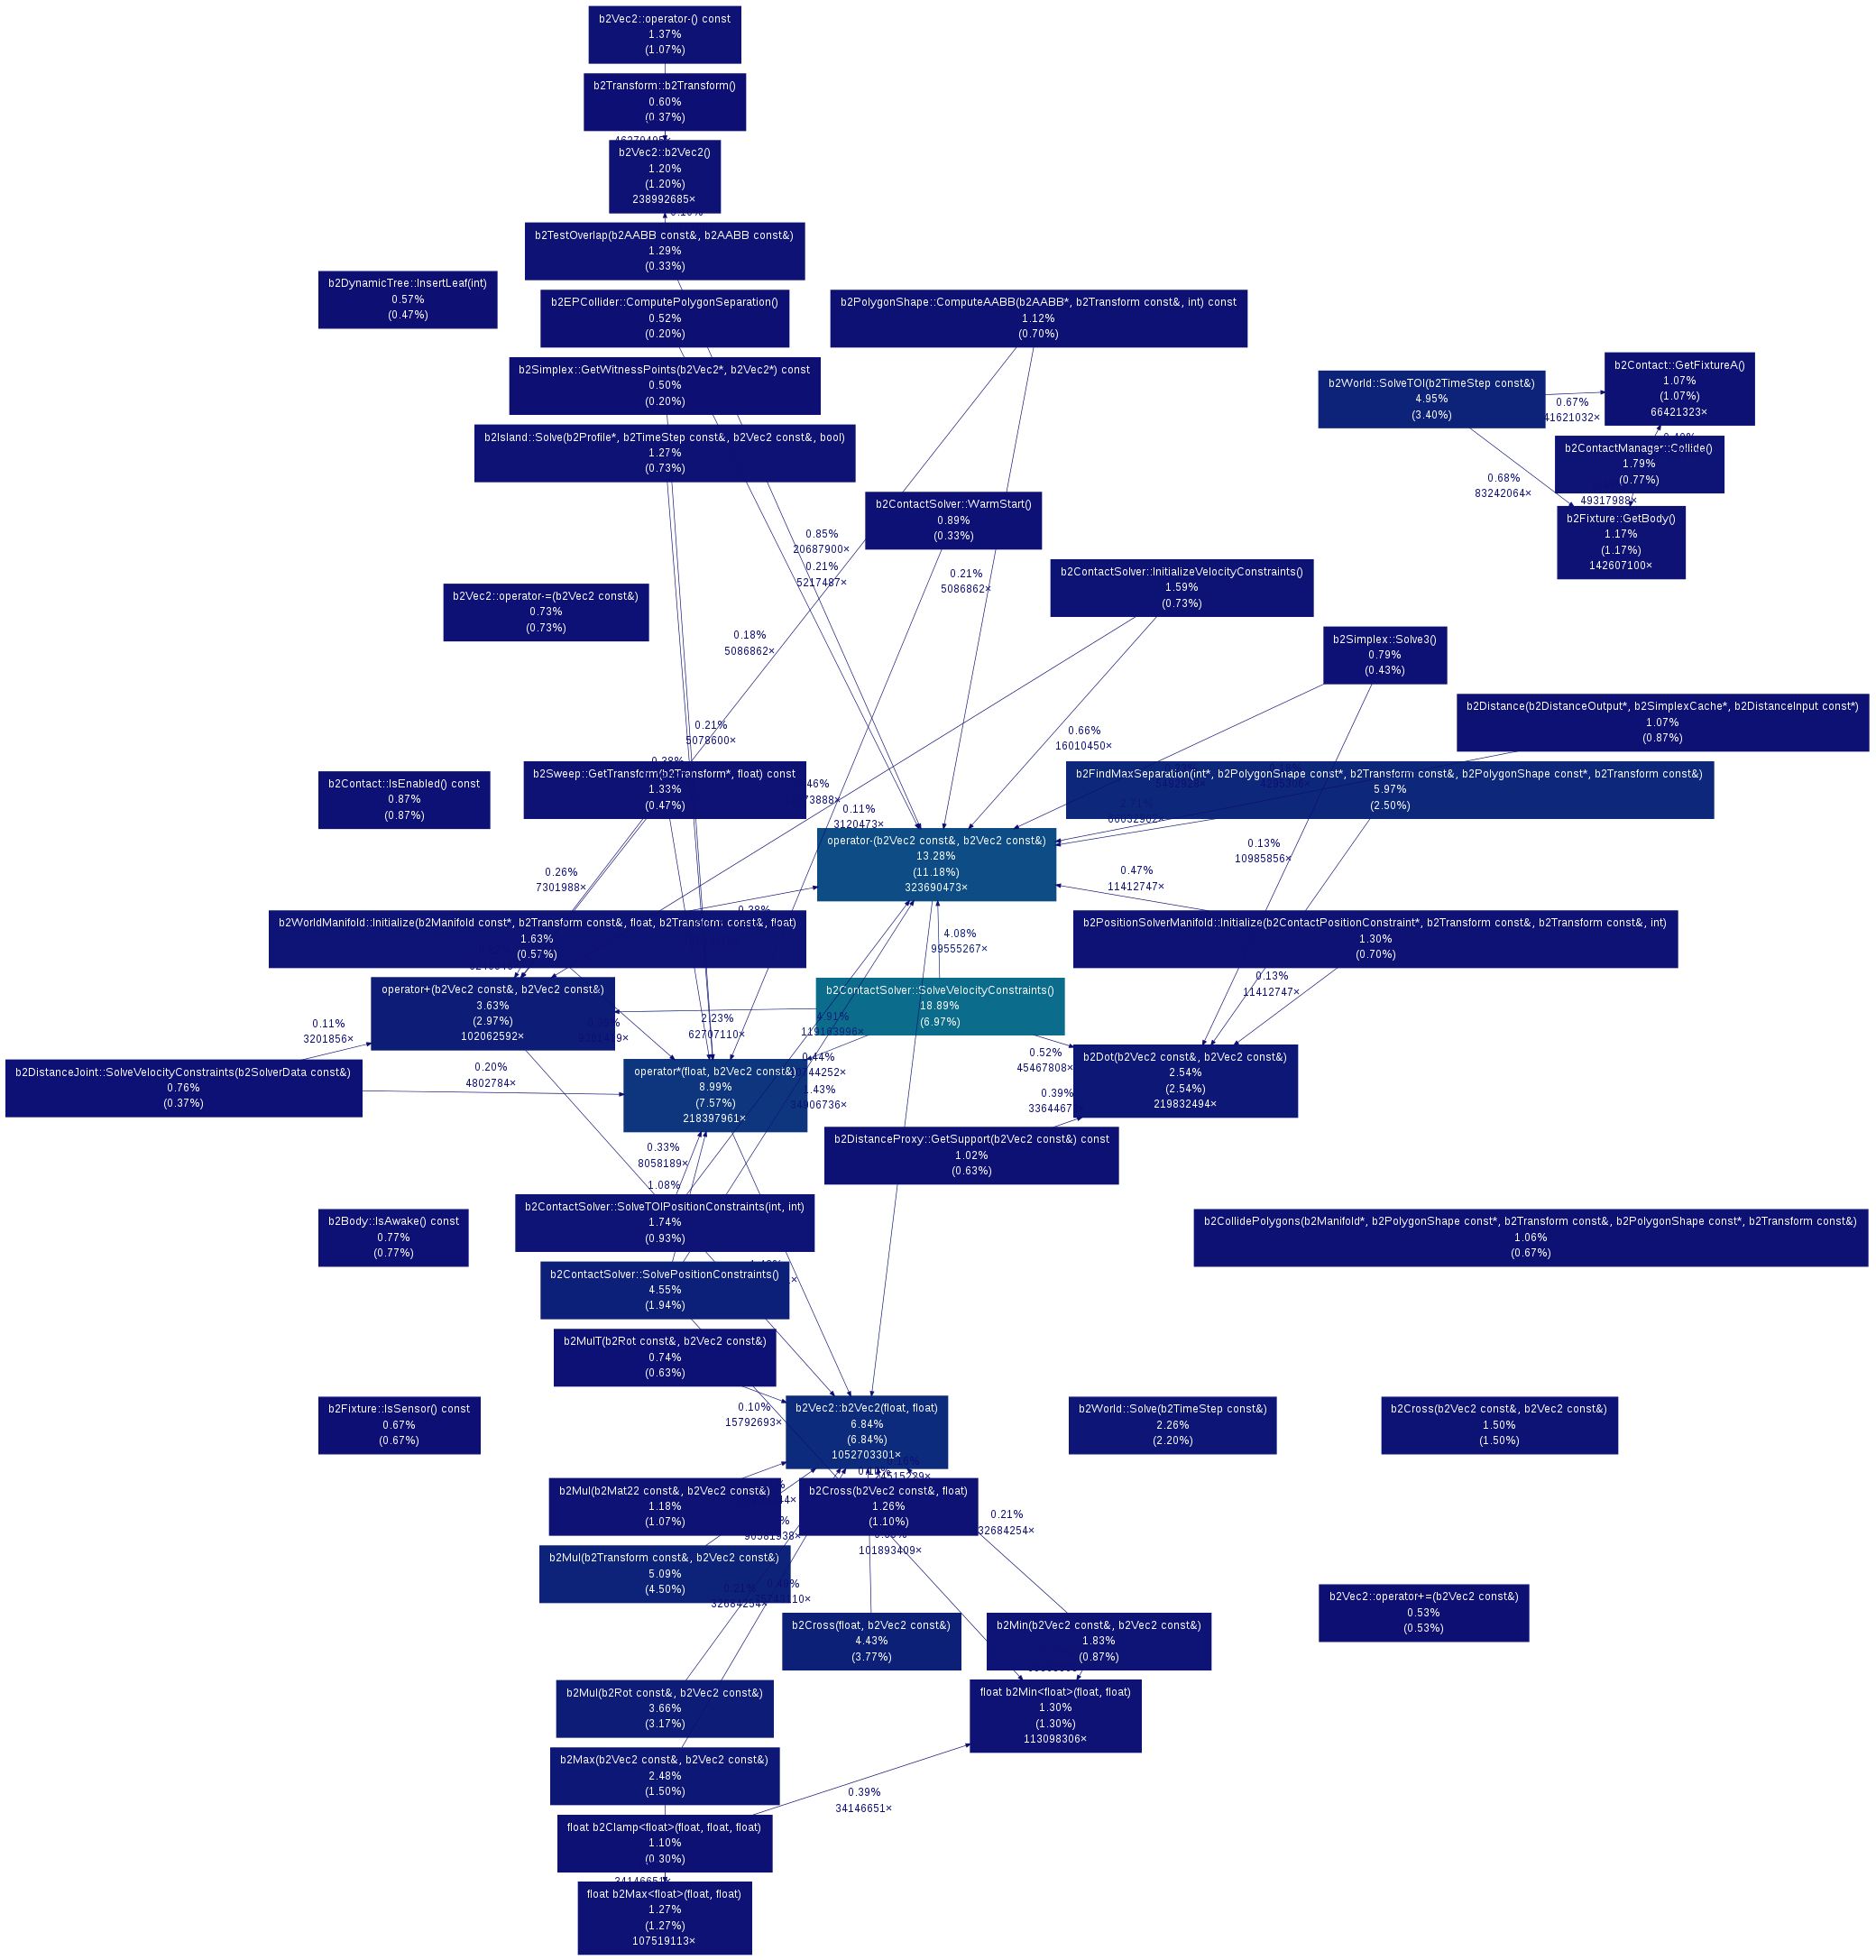
\includegraphics[scale=0.1]{../details/images/release.png}
\end{center}
The first thing we notice while observing the call graph is that it is a flowchart of functions called in order.Each block is representing a function with the name of the corresponding function and the time taken up by CPU in performing the function (in the form of percentage) is indicated in the box itself.The boxes are coloured according to the percentage time consumed.The arrows drawn between these boxes are representaion of which function call which one.If function A calls function B,then there is an arrow from A to B.Also, the arrows are indexed with number of times the call is done and also the amount of time spent in the function call.

\section{Difficulties arising with the initial design}
The initial design thought of was of much more complexity than we could do in box2d ie., it consists of many small parts whose behaviour cannot be exactly be depicted using Box2D.\\
The mechanism for the working of trigger was slightly modified to suit with the natural simulation of Box2D.

\bibliographystyle{plain}
\bibliography{project}
\end{document}
